\documentclass[varwidth=true, border=10pt, convert={size=1024x}]{standalone}
\usepackage{tikz}
\usetikzlibrary{spy,arrows}
\usepackage[detect-all]{siunitx}
\usepackage{calc}
%\usepackage{fontspec}
\usepackage{amsmath,amssymb}
%\usepackage{mathspec}
\usepackage{relsize}
\usetikzlibrary{calc}
\usepackage{exscale}
\usepackage{amsmath}
\definecolor{fillcolor}{HTML}{A8E6CE}
\usepackage{pgfplots}
\tikzset{>=latex}

\begin{document}
{\centering
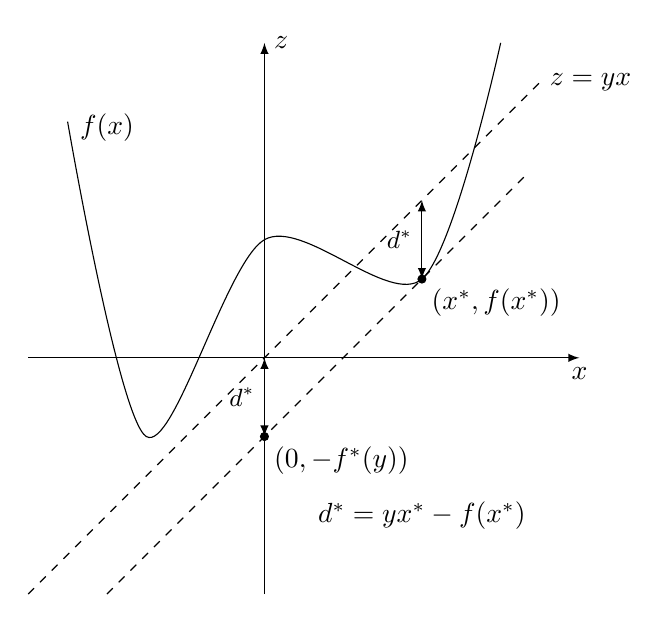
\begin{tikzpicture}[scale=1.]
	\draw[->] (-3,0) -- (4,0) node[below] {$x$};
    \draw[->] (0,-3) -- (0,4) node[right] {$z$};
      \draw plot [smooth] coordinates {(-2.5, 3 ) (-1.5, -1) (0, 1.5) (2, 1) (3, 4)};
      %\draw coordinates {(-3, 3)} node {$f(x)$};
      \draw[domain=-3:3.5,smooth,variable=\x,black, dashed] plot ({\x},{\x}) node[right] {$z = yx$};
      \node[label={$f(x)$}] at (-2, 2.5) {};
      \draw[domain=-2:3.3,smooth,variable=\x,black, dashed] plot ({\x},{\x - 1}); 
      \draw[fill] (2, 1) circle (.5mm) node[below right] {$(x^*, f(x^*))$};
      \draw[fill] (0, -1) circle (.5mm) node[below right] {$(0, -f^*(y))$};
      \draw[<->] (2, 1) -- node[left] {{\small $d^*$}} (2, 2) ;
      \draw[<->] (0, 0) -- node[left] {{\small $d^*$}} (0, -1);
      \node at (2, -2) {$d^* = yx^* - f(x^*)$};
      
\end{tikzpicture}
}
\end{document}